\documentclass{beamer}

\mode<presentation>
{
  \usetheme{CambridgeUS}
  \setbeamercovered{transparent}
}

\usepackage[english]{babel}
\usepackage[latin1]{inputenc}
\usepackage{times}
\usepackage[T1]{fontenc} 
% Or whatever. Note that the encoding and the font should match. If T1
% does not look nice, try deleting the line with the fontenc.
\usepackage{amsmath}

\newcommand{\linespace}{\vskip 0.25cm}

\definecolor{MyForestGreen}{rgb}{0,0.7,0} 
\newcommand{\tableemph}[1]{{#1}}
\newcommand{\tablewin}[1]{\tableemph{#1}}
\newcommand{\tablemid}[1]{\tableemph{#1}}
\newcommand{\tablelose}[1]{\tableemph{#1}}

\definecolor{MyLightGray}{rgb}{0.6,0.6,0.6}
\newcommand{\tabletie}[1]{\color{MyLightGray} {#1}}

% The text in square brackets is the short version of your title and will be used in the
% header/footer depending on your theme.
\title[Automatic Chord Recognition from Audio]{Automatic Chord Recognition from Audio}

% Sub-titles are optional - uncomment and edit the next line if you want one.
% \subtitle{Why does sub-tree crossover work?} 

% The text in square brackets is the short version of your name(s) and will be used in the
% header/footer depending on your theme.
\author[Emmons]{Alex Ray Emmons}

% The text in square brackets is the short version of your institution and will be used in the
% header/footer depending on your theme.
\institute[U of Minn, Morris]
{
  Division of Science and Mathematics \\
  University of Minnesota, Morris \\
  Morris, Minnesota, USA
}

% The text in square brackets is the short version of the date if you need that.
%\date[July '09, GECCO, Montr\'{e}al] % (optional)
%{10 July 2009 \\ GECCO, Montr\'{e}al}

% Delete this, if you do not want the table of contents to pop up at
% the beginning of each subsection:
\AtBeginSection[]
{
  \begin{frame}<beamer>
    \frametitle{Outline}
    \tableofcontents[currentsection, hideothersubsections]
  \end{frame}
}

\begin{document}

\begin{frame}
  \titlepage
\end{frame}

% For a 20-25 minute senior seminar talk you probably want something like:
% - Two or three major sections (other than the summary).
% - At *most* three subsections per section.
% - Talk about 30s to 2min per frame. So there should probably be between
%   15 and 30 frames, all told.

\section*{Overview}

\subsection*{The Big Picture}

\begin{frame}
  \frametitle{The Big Picture}
  

  \begin{itemize}
  	%\item Automatic chord recognition: extracting chord information from audio
	\item Used by researchers in the area of Music Information Retrieval (MIR) for tasks such as key detection, genre classification, and lyric interpretation. 
	\item \textbf{Problem:} Performing chord analysis from audio by hand is time consuming and prone to error.
	\item \textbf{Potential Solution:} Automatic chord recognition systems.
	\item \textbf{Issues:} Noise in recordings, determining where chords change, complex music.
%	\item \textbf{Solution:} Different combinations of feature extraction and pattern matching, preprocessing the audio signal to reduce noise, and segmenting it by beat.
  \end{itemize}

   
%       \\
%    \only{\tiny{Bluedrakon \\ \url{http://tr.im/pWUi} }}

\end{frame}

\begin{frame}
	\frametitle{Solution}
	
	\begin{itemize}
		\item Feature Extraction: Audio signals are processed to extract harmonic information, represented using a Pitch Class Profile.
		\item Pattern Matching: Chord labels are applied by matching chord models to the features that are present in the audio. 
		\item Models can be generated either by hand or stochastically.
	\end{itemize}
	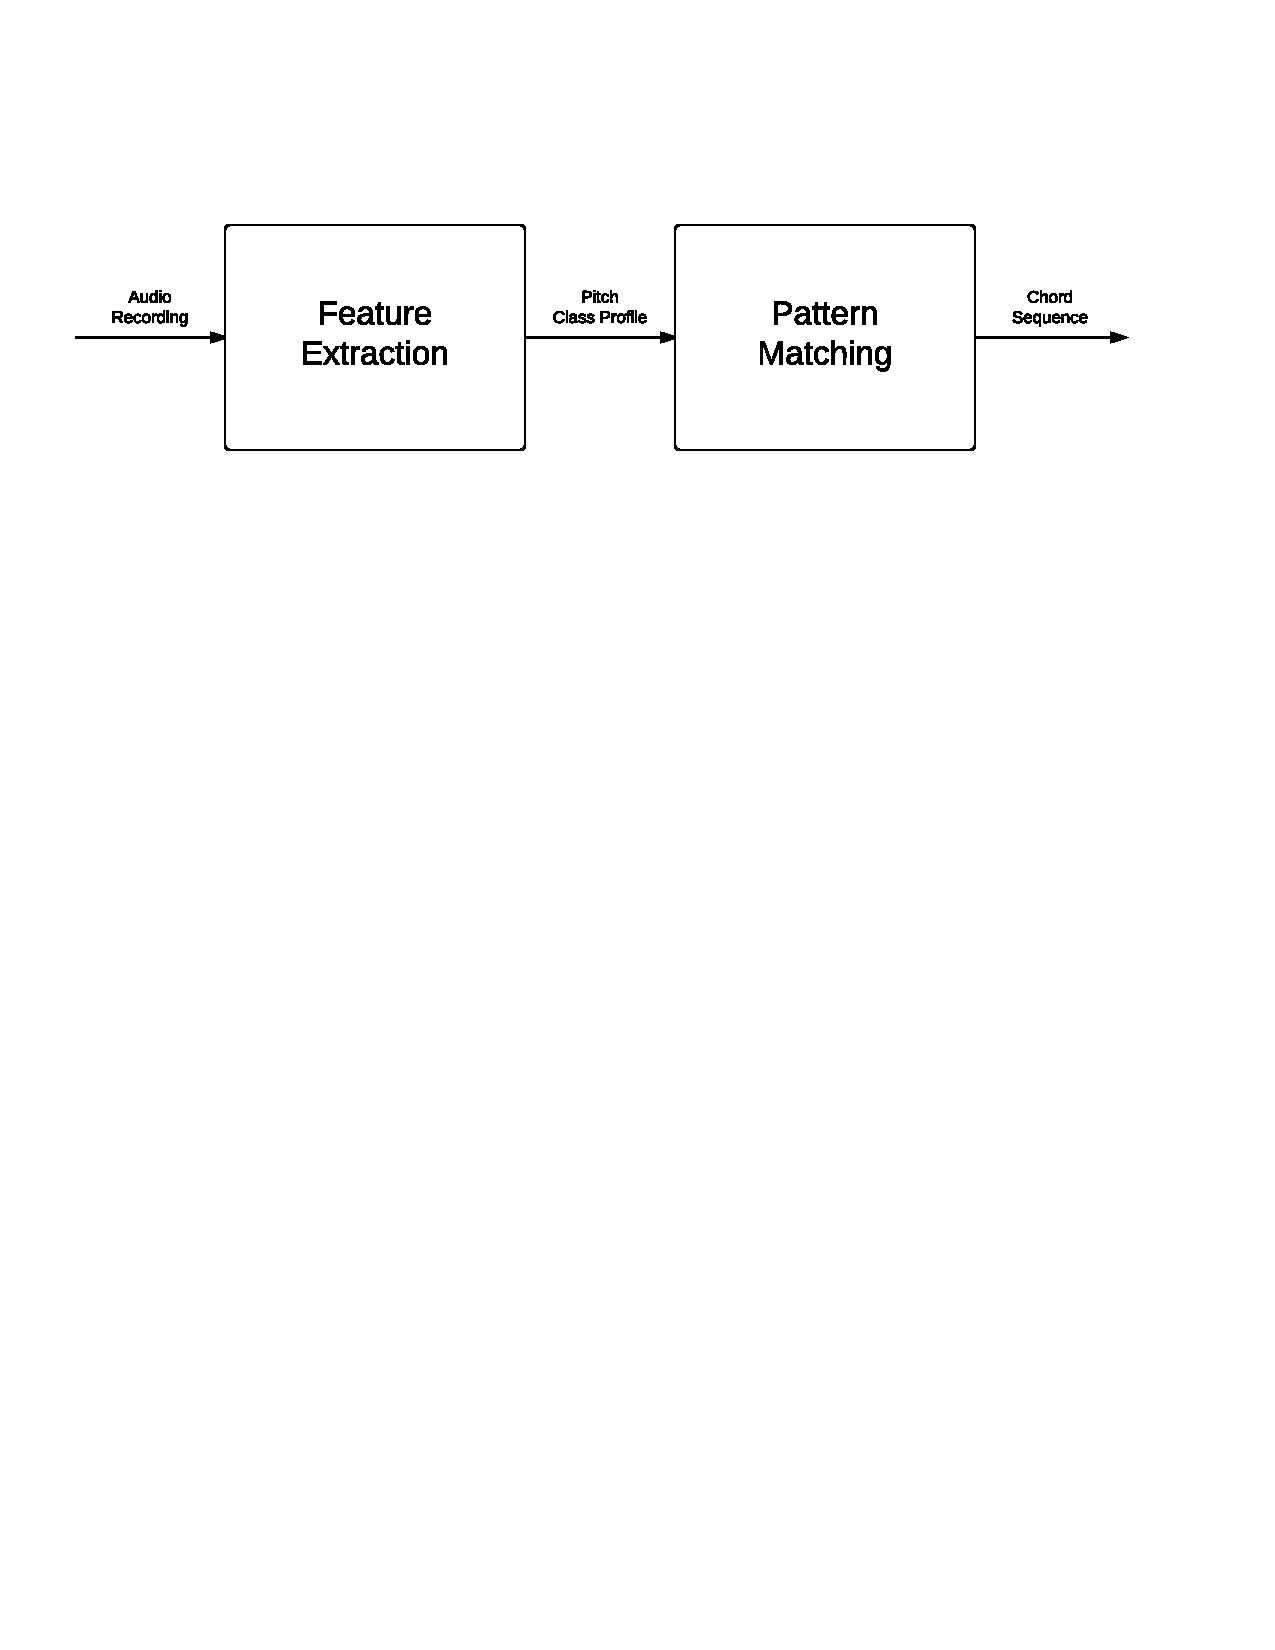
\includegraphics[width=0.95\textwidth]{ChordRecognition.pdf}
\end{frame}

\subsection*{Outline}

\begin{frame}
  \frametitle{Outline}
  \tableofcontents[hideallsubsections]
\end{frame}

\section[Feature Extraction]{Feature Extraction}

%\begin{frame}
%	\frametitle{Feature Extraction}
%\end{frame}

\subsection{Preprocessing}

\begin{frame}
	\frametitle{Preprocessing}
	
	\begin{itemize}
		\item Preprocessing is an optimization step, performed during feature extraction, before a Pitch Class Profile (PCP) is generated.
		\item The goal of preprocessing is to remove as much background noise as possible from the audio file in an effort to provide a smooth and clear PCP.
		\item Two issues, background noise and overtones, usually addressed separately.
	\end{itemize}
\end{frame}	

\subsection{Pitch Class Profile}

\begin{frame}
  \frametitle{Pitch Class Profile}
  \begin{itemize}
  \item Pitch Class Profile (PCP) measures energy in the 12 frequency regions where musical notes occur.
  \item Each row represents a pitch class, or note, and each column represents a frame, or period of time.
  \item Actual chord progression is shown above for reference.
  \end{itemize}


%\linespace

%Chords are determined by note values regardless of height, or octave, so this method is ideal. 

%\linespace
 



 \begin{center}
 %put PCP diagram here
   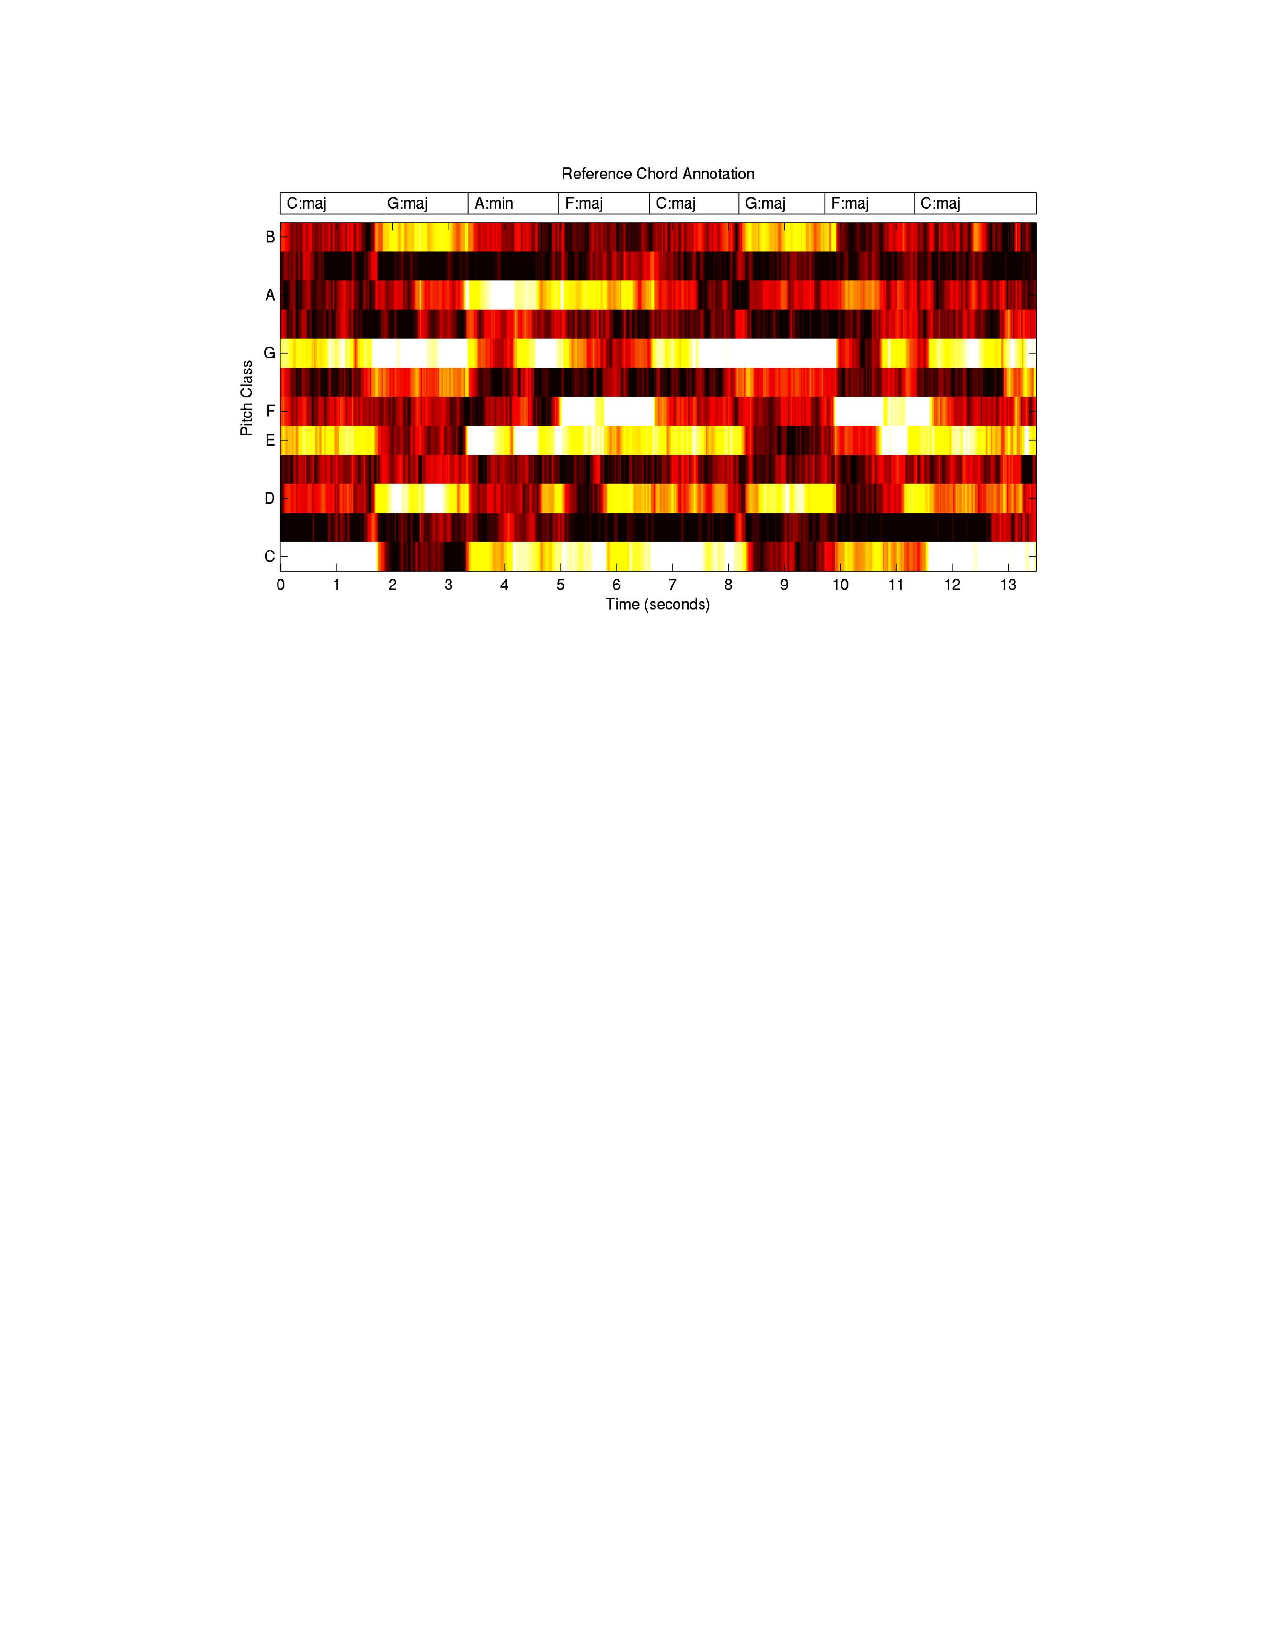
\includegraphics[width=.70\textwidth]{fig4.pdf}
%   \\
%   \tiny{Sam Fraser-Smith \\ \url{http://tr.im/pq7l} }
 \end{center}

\end{frame}



\section[Pattern Matching]{Pattern Matching}

\subsection{Hidden Markov Models}

\begin{frame}
	\frametitle{Hidden Markov Models}
	\begin{columns}
	\begin{column}{.6\textwidth}
		\begin{itemize}
			\item A Hidden Markov Model (HMM) describes a sequence of states and transition probabilities.
			\item Transition probabilities are learned from labeled training data.
			\item The chords for the testing data are unknown, or hidden states. The PCP frames are the observed states.
			\item Observed states and transition probabilities are used to find the most likely sequence and eliminate unlikely transitions.
		\end{itemize}
	\end{column}
	\begin{column}{.4\textwidth}
		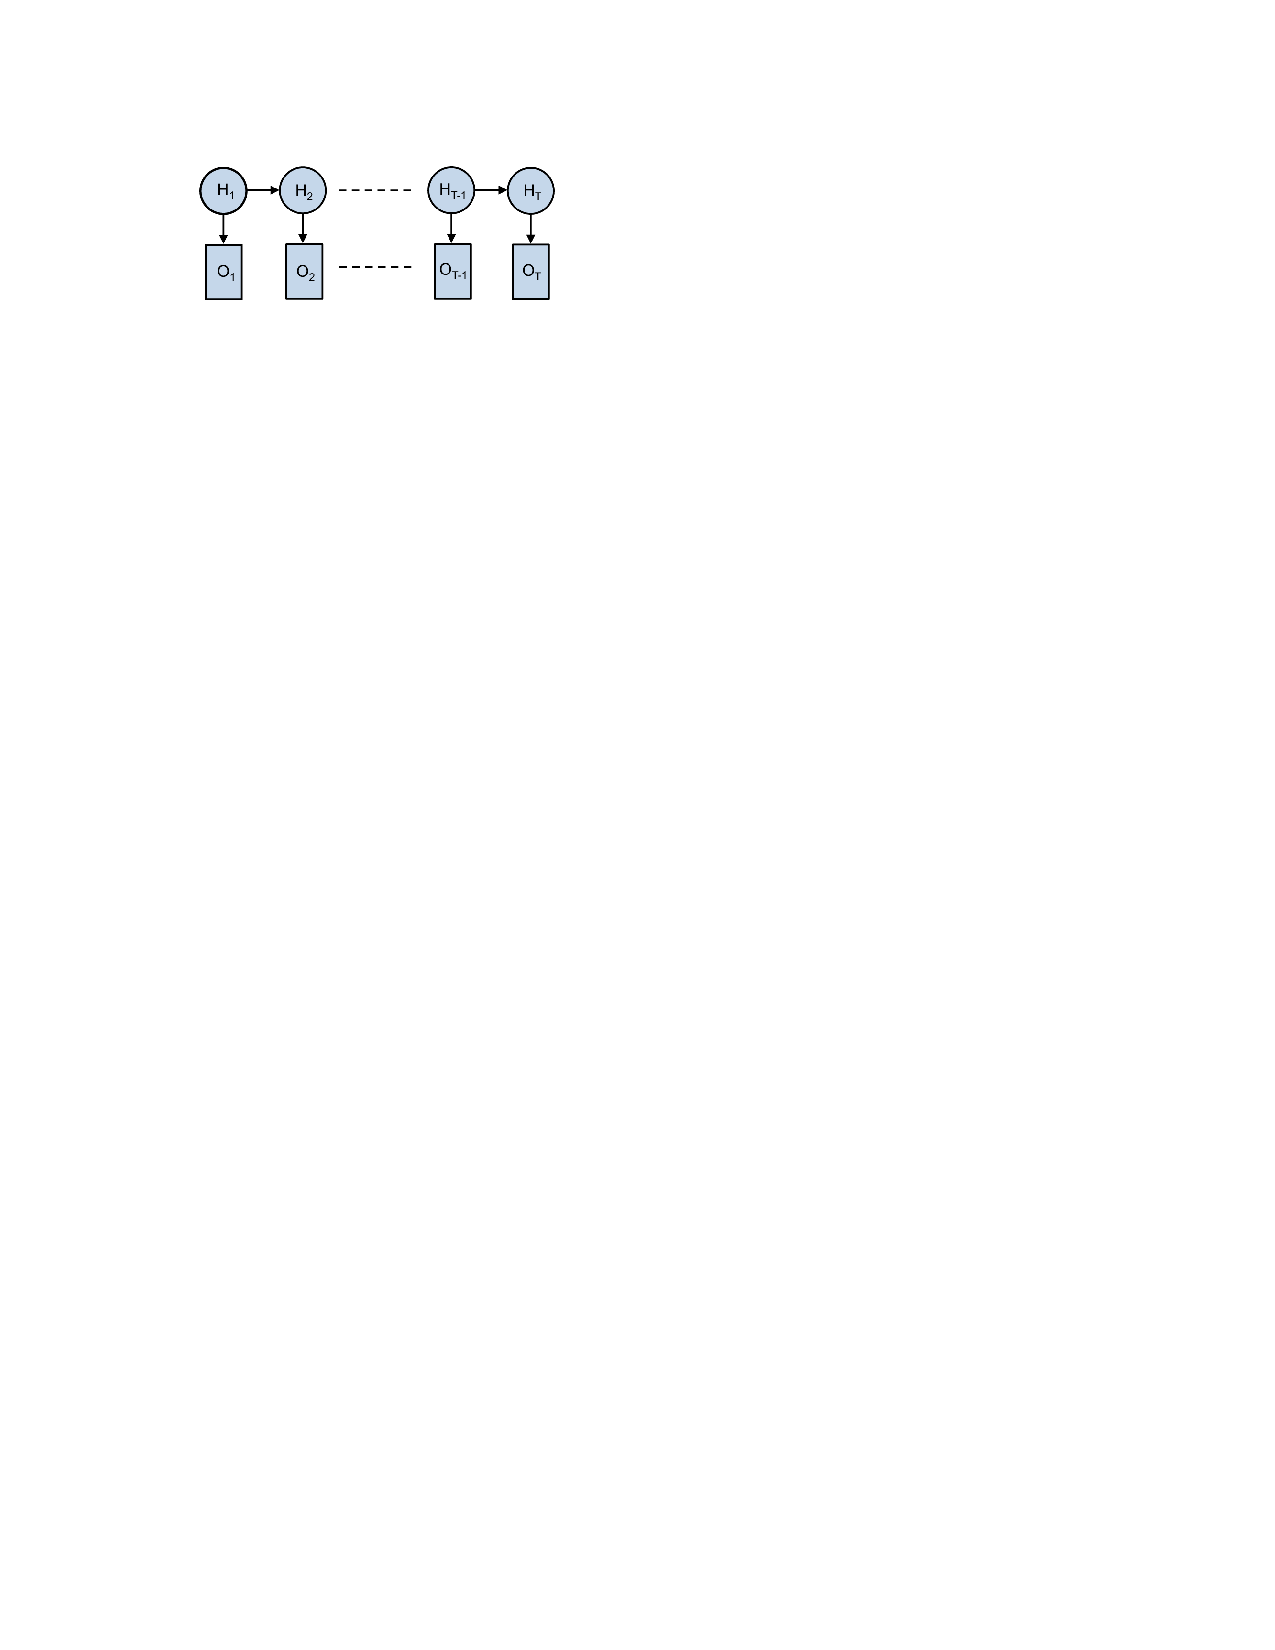
\includegraphics[width=.95\textwidth]{hmm.pdf}
	\end{column}
	\end{columns}
\end{frame}

\begin{frame}
	\frametitle{Hidden Markov Models}
	
	\begin{columns}
	\begin{column}{.6\textwidth}
		\begin{itemize}
			\item Transition probabilities are learned by dividing the transitions to each chord by the total transitions from that chord.
			\item This is done for each chord, assigning a probability to all possible transitions.
%			\item The Viterbi algorithm is used to find the most likely sequence and eliminate unlikely transitions.
		\end{itemize}
	\end{column}
	\begin{column}{.4\textwidth}
	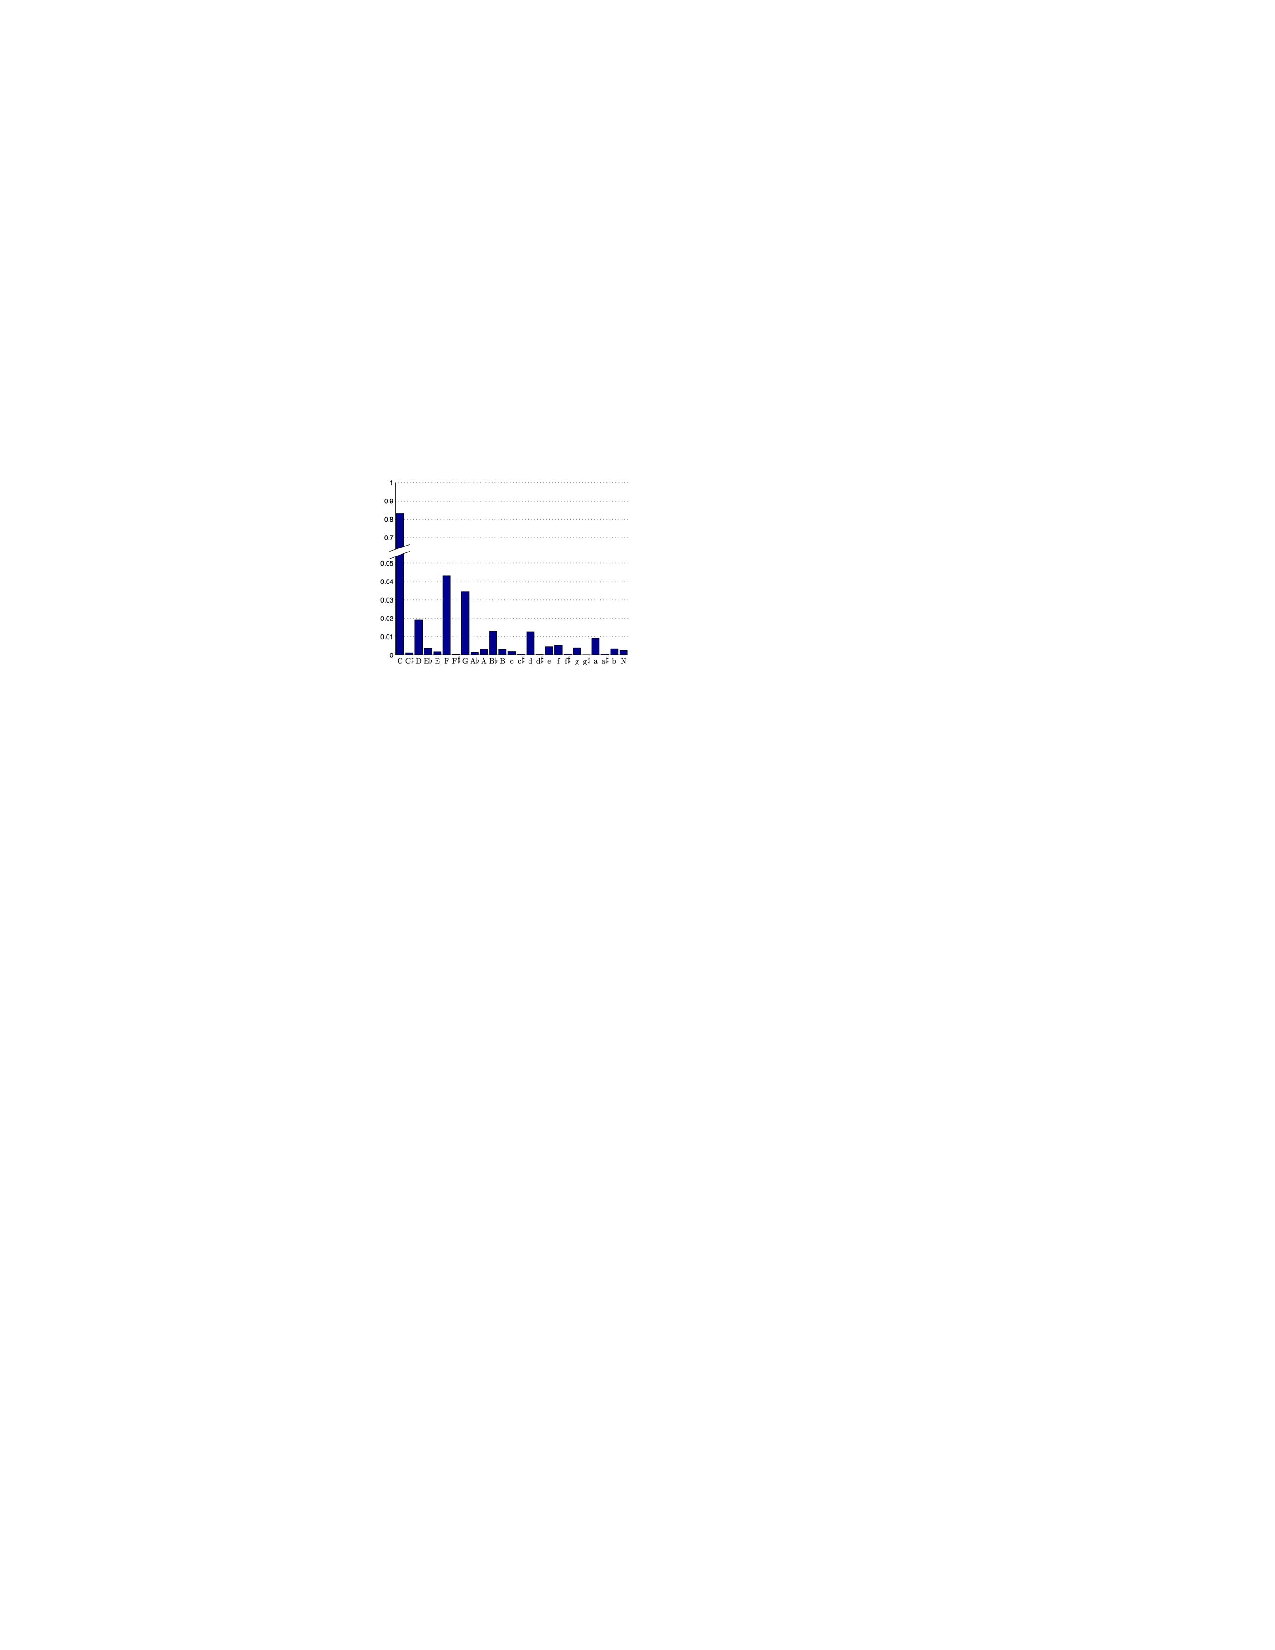
\includegraphics[width=.95\textwidth]{transitionProbabilities.pdf} \\
	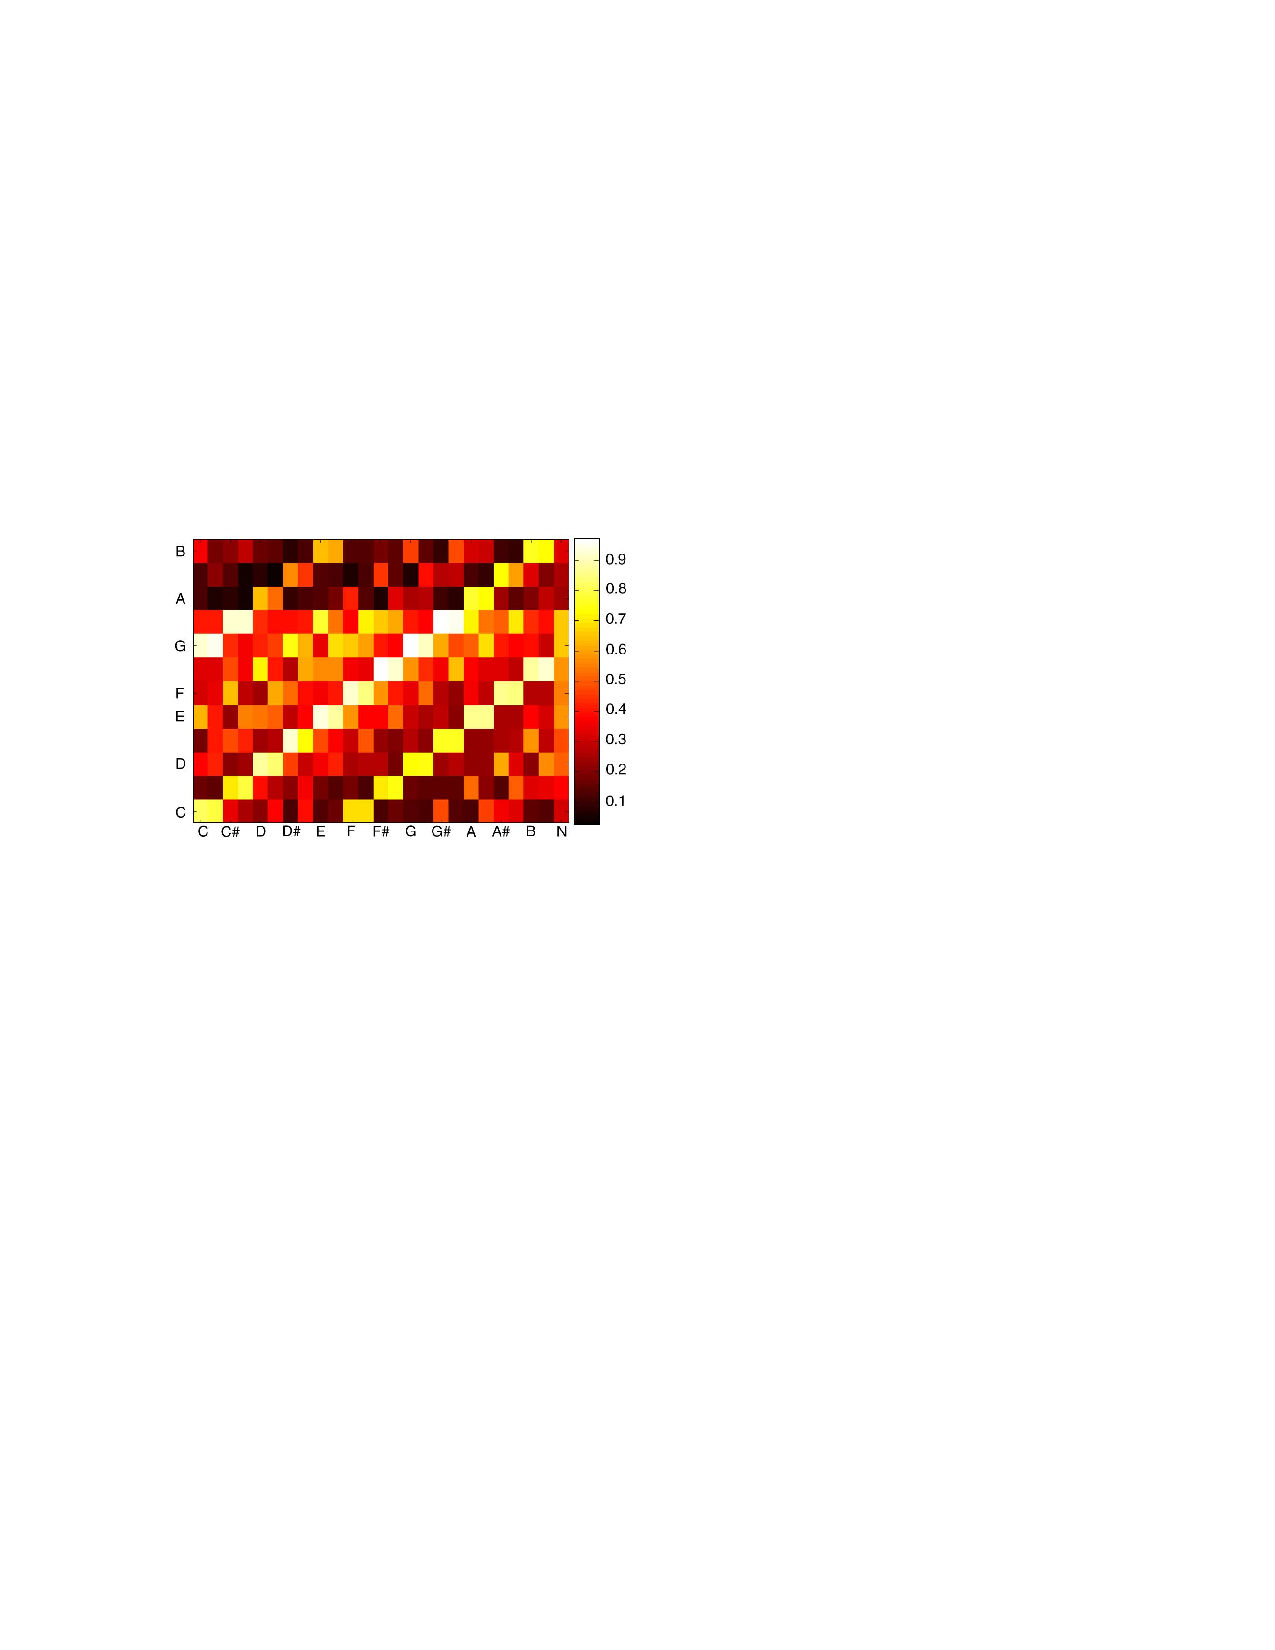
\includegraphics[width=.95\textwidth]{transitionProbabilities2.pdf}
	\end{column}
	\end{columns}
\end{frame}

\subsection{Gaussian Mixture Models}

\begin{frame}
	\frametitle{Gaussian Mixture Models}
	\begin{itemize}
		\item More detailed models for each chord are created by averaging features from multiple PCPs.
		\item Multiple variations of the same chord are represented using multiple Gaussian components.
		\item Like HMM, labeled training data is used and transition probabilities are learned for each chord.
		\item The observed chord is matched with each chord model to find the best fit.
		
	\end{itemize}
\end{frame}

\subsection{Support Vector Machines}

\begin{frame}
	\frametitle{Support Vector Machines}
	\begin{itemize}
		\item Another type of supervised learning system. 
		\item Trained with labeled testing data, chord labels are applied to segments of the test data.
		\item Only works on the kind of data it is trained on. 
		\item Training procedure is complex for large datasets.
	\end{itemize}
\end{frame}

\section[Research Cases]{Research Cases}

\subsection[Case 1: Effects of Proper Signal Processing]{Case 1: Effects of Proper Signal Processing}

\begin{frame}
  \frametitle{Case 1: Effects of Proper Signal Processing}
	\begin{itemize}
		\item Two methods of preprocessing were used.
		\item Four feature vectors were compared.
		\item Two datasets were used.
		\item GMMs and SVMs are compared.
	\end{itemize}
 
 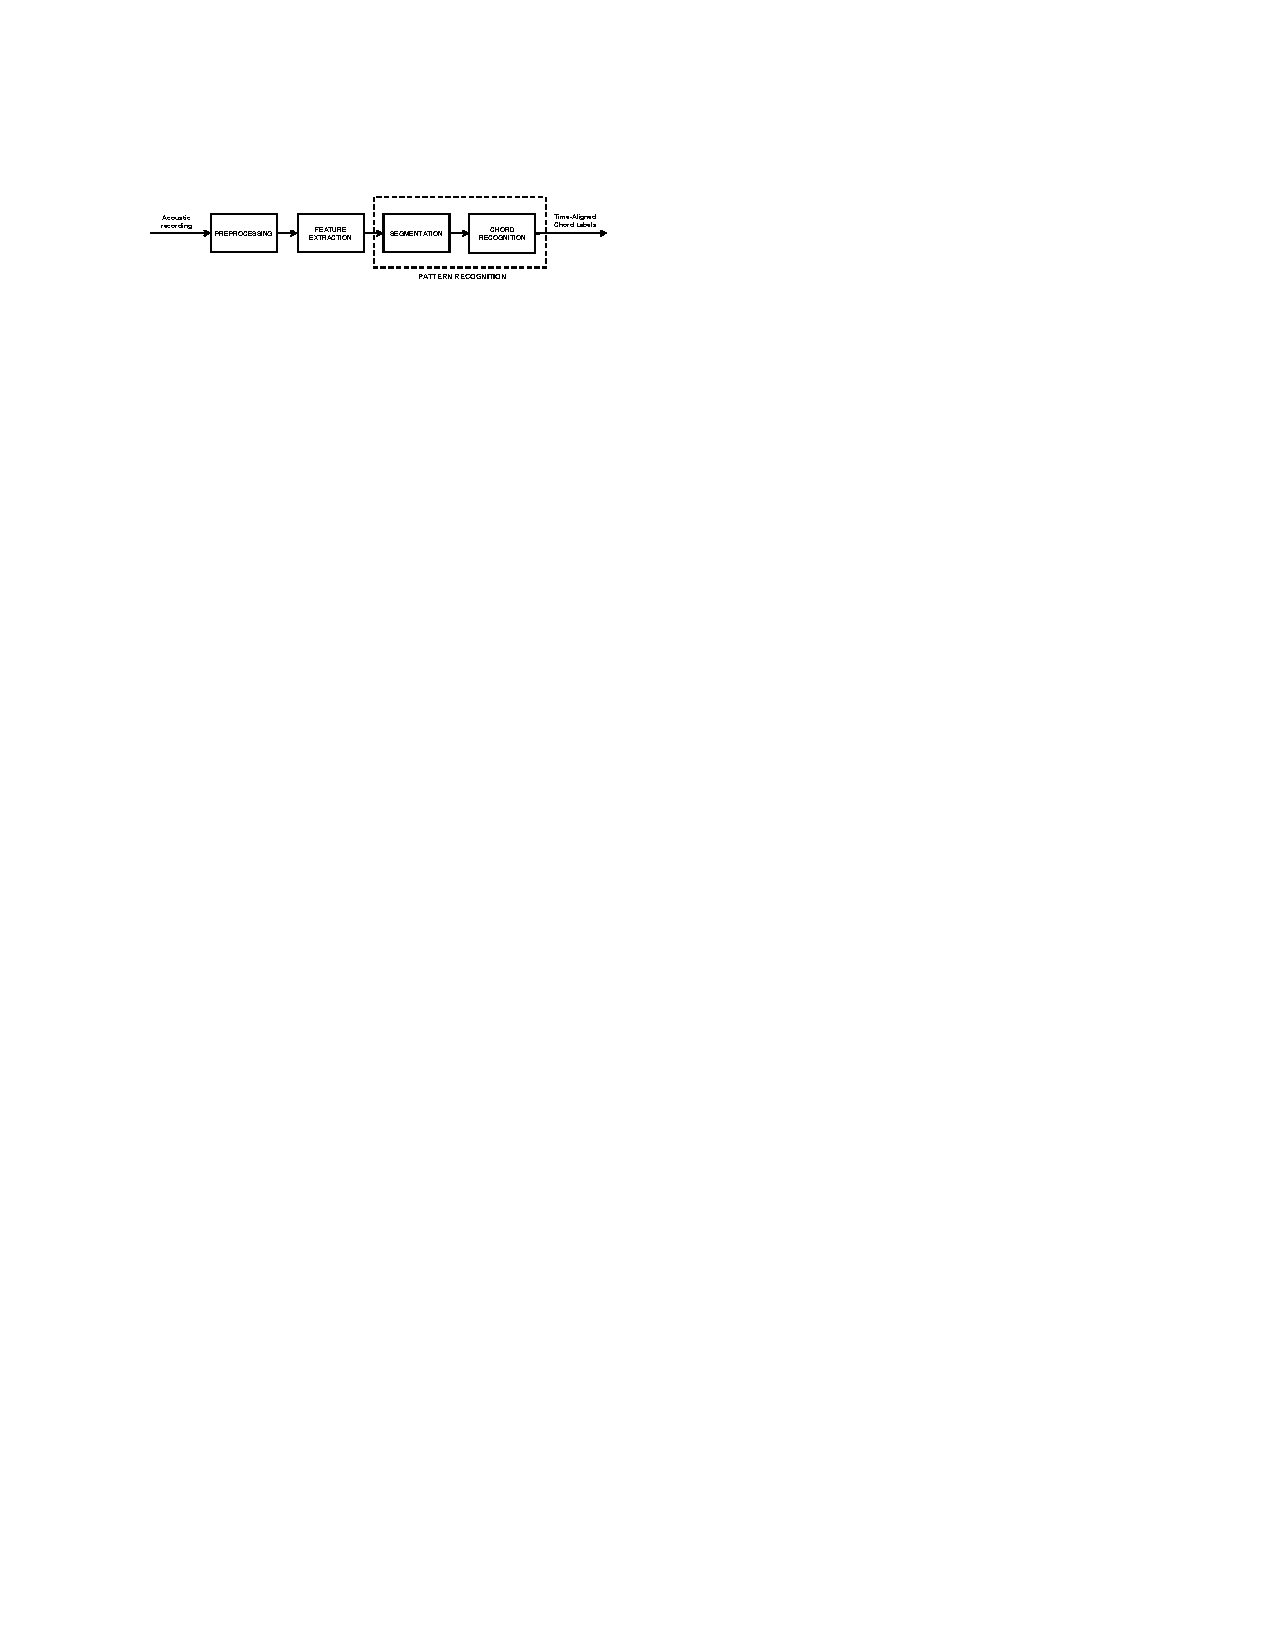
\includegraphics[width=0.95\textwidth]{fig2.pdf}
\end{frame}

\begin{frame}
	\frametitle{Preprocessing}
	\begin{columns}
	\begin{column}{.5\textwidth}
	\begin{itemize}
	\item Homomorphic Liftering: Finds strong peaks in the frequency areas where notes occur.
		\item Harmonic Product Spectrum (HPS): De-emphasizes overtones, emphasizes chord tones.
	\end{itemize}
	\end{column}
	\begin{column}{.5\textwidth}
	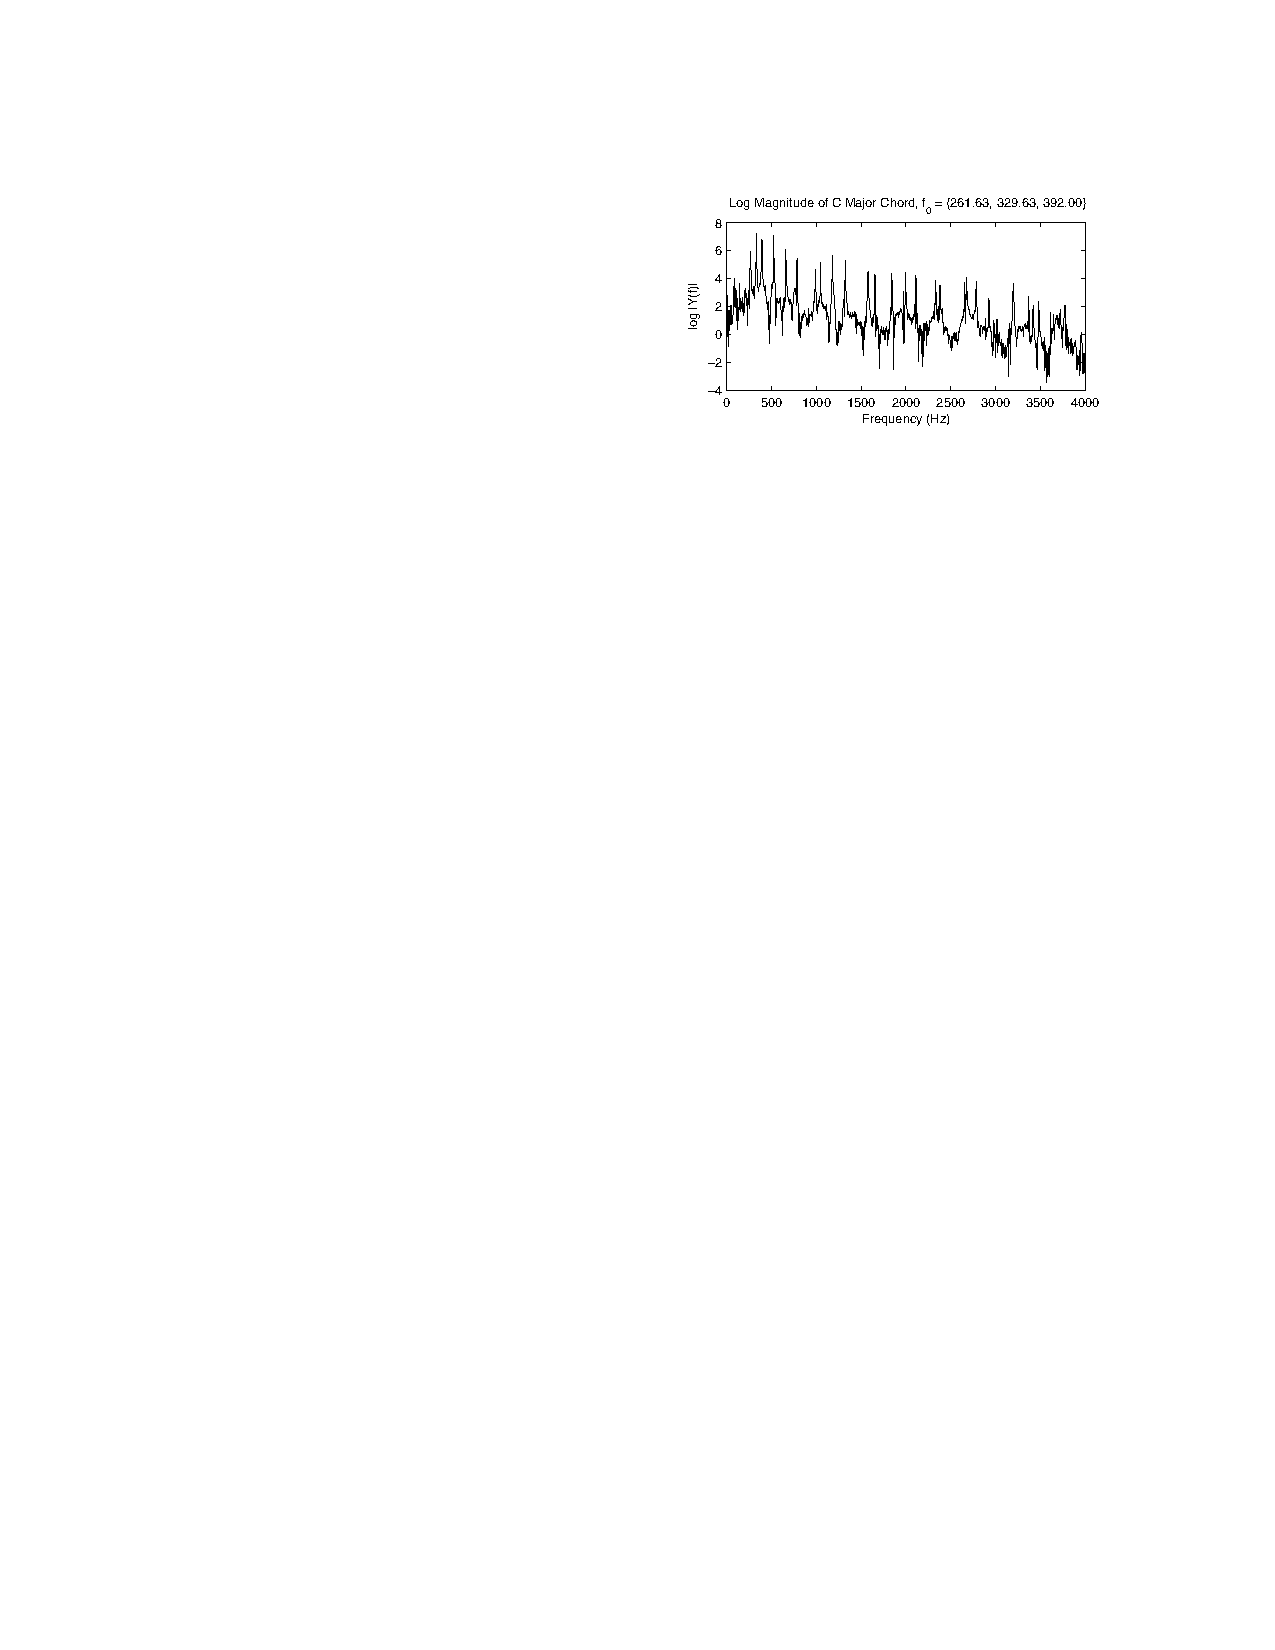
\includegraphics[width=0.70\textwidth]{freq.pdf} \\
	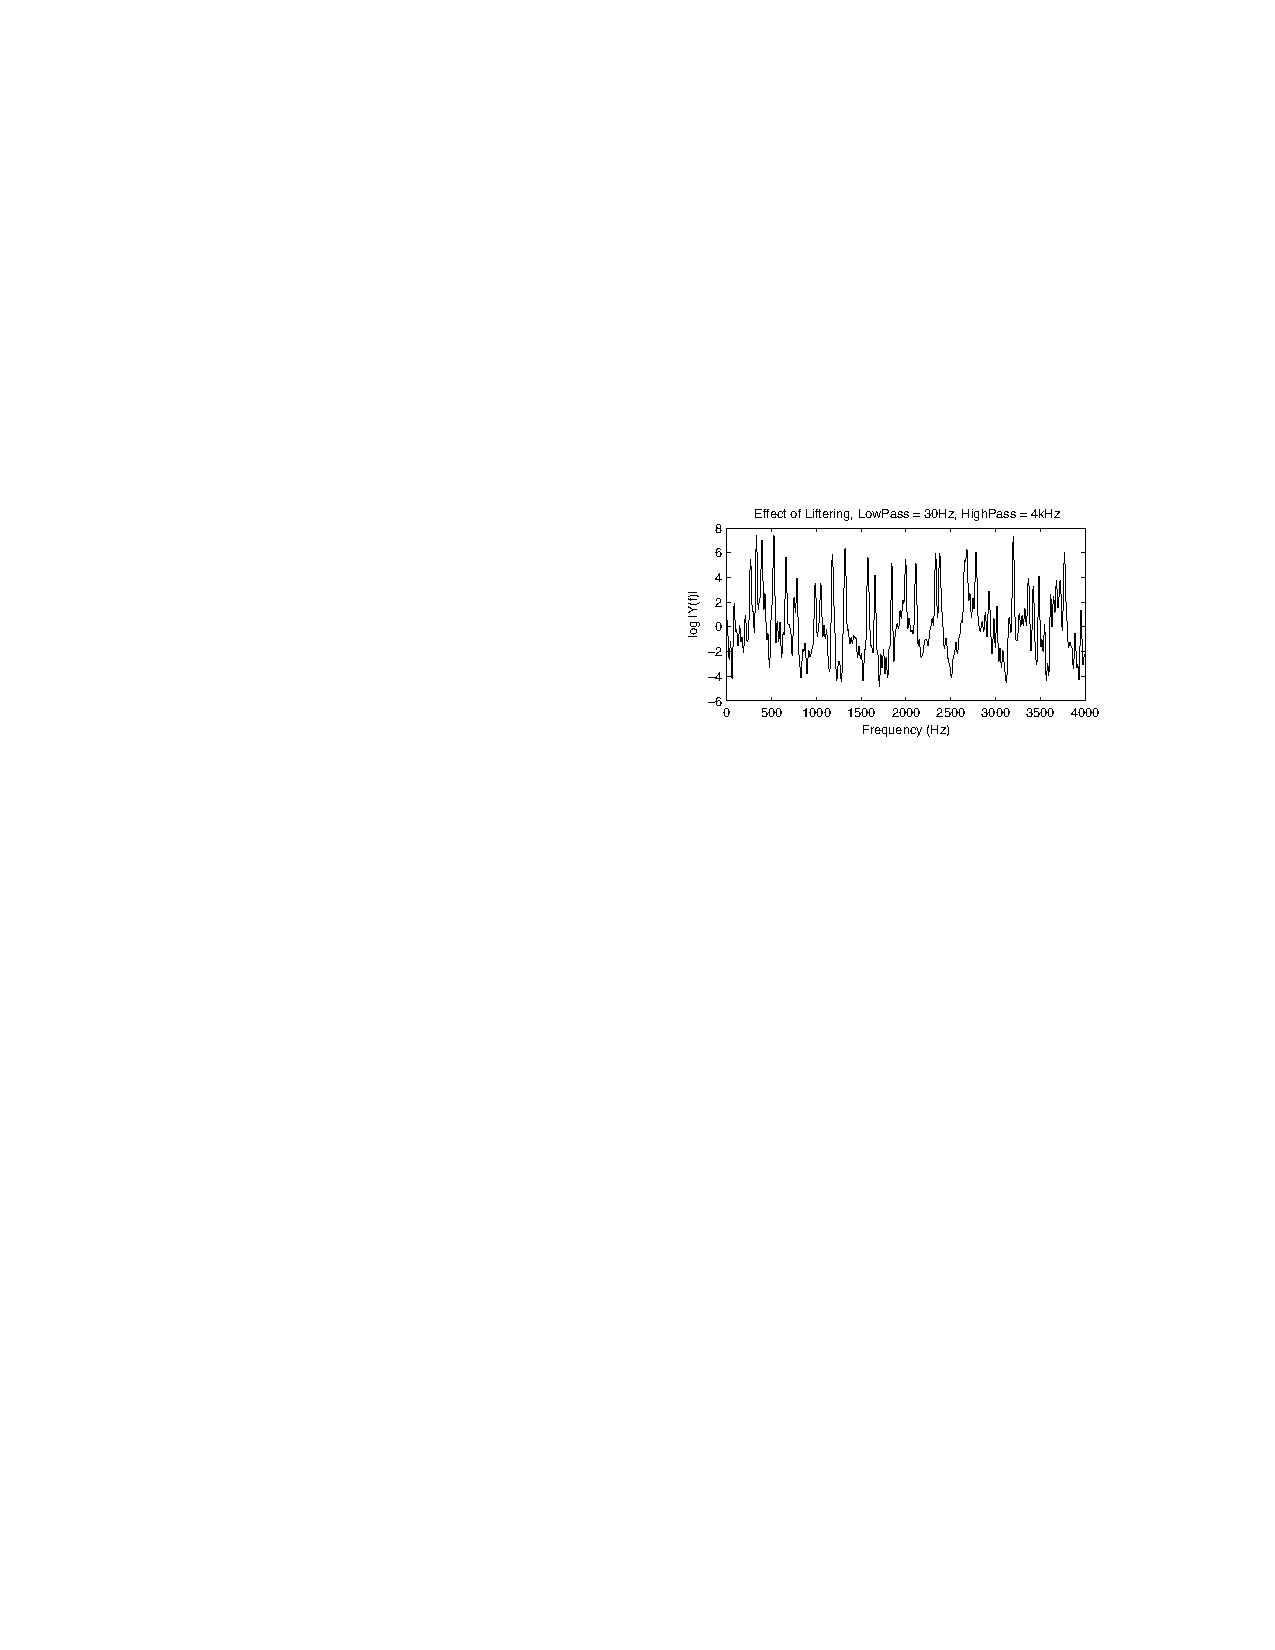
\includegraphics[width=0.70\textwidth]{freq2.pdf} \\
	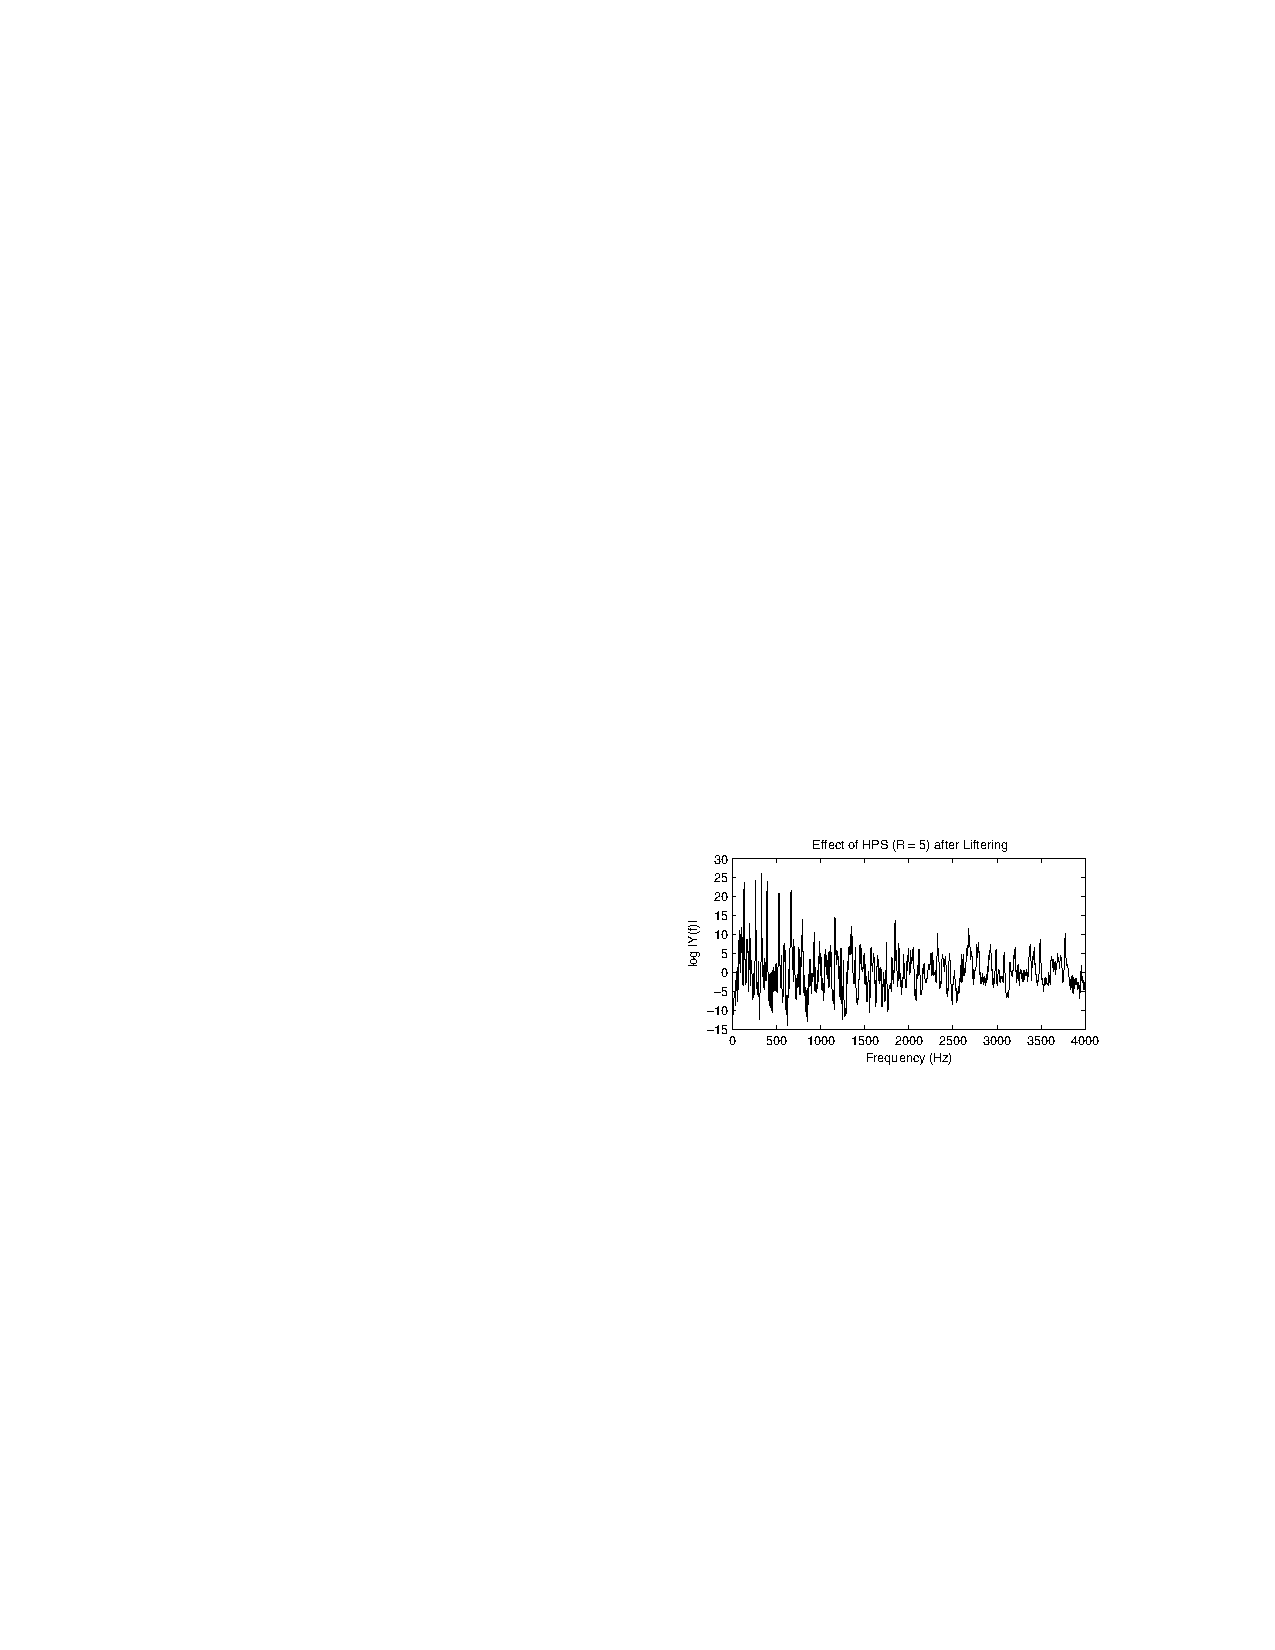
\includegraphics[width=0.70\textwidth]{freq3.pdf}
	\end{column}
	\end{columns}
\end{frame}

\begin{frame}
	\frametitle{Feature Extraction}
	 \begin{itemize}
 	\item Four Feature Vectors (FV), or combinations of methods used for feature extraction were compared.
 	\item Sample Rate is the audio resolution and Fast Fourier Transform (FFT) determines the resolution in the frequency domain. 
 \end{itemize}
 
	\begin{table}
\centering
\begin{tabular}{|c|c|c|c|c|c|} \hline
 & \textbf{Type} & \textbf{Sample Rate} & \textbf{FFT Length} & \textbf{Liftering} & \textbf{HPS Ratio} \\ \hline
\textbf{FV1} & FB & 44100 & 32768 & yes & 5 \\ \hline
\textbf{FV2} & PCP & 11025 & 4096 & no & 1 \\ \hline
\textbf{FV3} & PCP & 44100 & 32768 & no & 1 \\ \hline
\textbf{FV4} & PCP & 44100 & 32768 & yes & 5 \\ \hline
\end{tabular}
%\caption{Feature Vectors, or combinations of methods used for feature extraction, for isolated chord recognition in research case 1~\cite{Morman:2006}.}
\label{tab:tab2}
\end{table} 
\end{frame}

\begin{frame}
	\frametitle{Datasets}
	\begin{columns}
	\begin{column}{.6\textwidth}
	\begin{itemize}
	\item \textbf{Isolated chord dataset:} 7790 chords synthesized from Musical Instrument Digital Interface (MIDI) data on piano and strings. 
	\item 80\% used for training, 20\% for testing. 3 complexity levels were tested.
 	\item \textbf{Continuous single-instrument audio:} 50 hymns from the Trinity Hymnal, a MIDI collection of 761 hymns.
 	\item 40 used for training, 10 for testing. FV4 and DS3 are used with an SVM.
	\end{itemize}
	\end{column}
	\begin{column}{.4\textwidth}
	\begin{table}
	\tiny
\centering
\begin{tabular}{|c|c|c|c|} \hline
&\multicolumn{3}{|c|}{\textbf{Label given in:}} \\ \hline
\textbf{Label} & \textbf{DS1} & \textbf{DS2} & \textbf{DS3} \\ \hline
Major & Major & Major & Major \\ \hline
Minor & Minor & Minor & Minor \\ \hline
Major 7 & - & Major & Major 7 \\ \hline
Minor 7 & - & Minor & Minor 7 \\ \hline
Dom. 7 & - & Major & Dom. 7 \\ \hline
Dim. & Dim. & Dim. & Dim. \\ \hline
Full Dim. & - & Dim. & Full Dim. \\ \hline
Half Dim. & - & Dim. & Half Dim. \\ \hline
Augmented & Aug. & Aug. & Augmented \\ \hline
Sus. 4 & - & - & Sus. 4 \\ \hline
7 Sus. 4 & - & - & 7 Sus. 4 \\ \hline
\end{tabular}
%\caption{Chord complexity levels used in research case 1~\cite{Morman:2006}.}
\label{tab:tab1}
\end{table} 
\end{column}
\end{columns}
\end{frame}  

\begin{frame}
	\frametitle{Results}
	
\begin{table}\small
\centering
\begin{tabular}{|c|c|c|c|} \hline
\textbf{Feature Vector} & \textbf{DS1} & \textbf{DS2} & \textbf{DS3} \\ \hline
\textbf{FV1} & 83.68 & 61.85 & 57.24 \\ \hline
\textbf{FV2} & 90.33 & 82.44 & 82.26 \\ \hline
\textbf{FV3} & \textbf{91.76} & \textbf{84.20} & \textbf{84.09} \\ \hline
\textbf{FV4} & 85.64 & 79.40 & 78.93 \\ \hline
\end{tabular}
\caption{Isolated chord recognition accuracy using GMM, training set: piano, testing set: piano}
\label{tab:tab3}
\end{table} 

\begin{table}\small
\centering
\begin{tabular}{|c|c|c|c|} \hline
\textbf{Feature Vector} & \textbf{DS1} & \textbf{DS2} & \textbf{DS3} \\ \hline
\textbf{FV1} & 68.06 & 42.00 & 33.62 \\ \hline
\textbf{FV2} & 42.72 & 18.60 & 16.30 \\ \hline
\textbf{FV3} & 43.49 & 22.00 & 18.31 \\ \hline
\textbf{FV4} & \textbf{86.94} & \textbf{80.23} & \textbf{80.18} \\ \hline
\end{tabular}
\caption{Isolated chord recognition accuracy using GMM, training set: piano, testing set: strings}
\label{tab:tab4}
\end{table}



\end{frame}

\begin{frame}
	\frametitle{Results}
	
\begin{table}\small
\centering
\begin{tabular}{|c|c|c|c|} \hline
\textbf{Feature Vector} & \textbf{DS1} & \textbf{DS2} & \textbf{DS3} \\ \hline
\textbf{FV1} & 93.43 & 88.21 & 86.52 \\ \hline
\textbf{FV2} & 94.78 & 93.26 & 93.13 \\ \hline
\textbf{FV3} & \textbf{95.23} & \textbf{94.31} & \textbf{94.24} \\ \hline
\textbf{FV4} & 90.56 & 88.08 & 87.74 \\ \hline
\end{tabular}
\caption{Isolated chord recognition accuracy using SVM, training set: piano, testing set: piano}
\label{tab:tab7}
\end{table}

\begin{table}\small
\centering
\begin{tabular}{|c|c|c|c|} \hline
\multicolumn{4}{|c|}{\textbf{Number of Scatter Points}} \\ \hline
\textbf{3} & \textbf{5} & \textbf{7} & \textbf{9} \\ \hline
72.73 & 87.77 & 88.07 & \textbf{88.42} \\ \hline
\end{tabular}
\caption{Continuous single-instrument recognition accuracy using FV4 and DS3, with varying number of scatter points}
\label{tab:tab8}
\end{table}

\end{frame}


\subsection[Case 2: HMM Trained with Audio from Symbolic Data]{Case 2: HMM Trained with Audio from Symbolic Data}

\begin{frame}
  \frametitle{Case 2: HMM Trained with Audio-From-Symbolic Data}
  \begin{columns}
	\begin{column}{.6\textwidth}
	\begin{itemize}
		\item Chord label data and audio files are created from the same MIDI data.
		\item Pitch Class profile is generated from the audio.
		\item These pieces are used to train a supervised HMM.
	\end{itemize}
	\end{column}
	\begin{column}{.4\textwidth}
  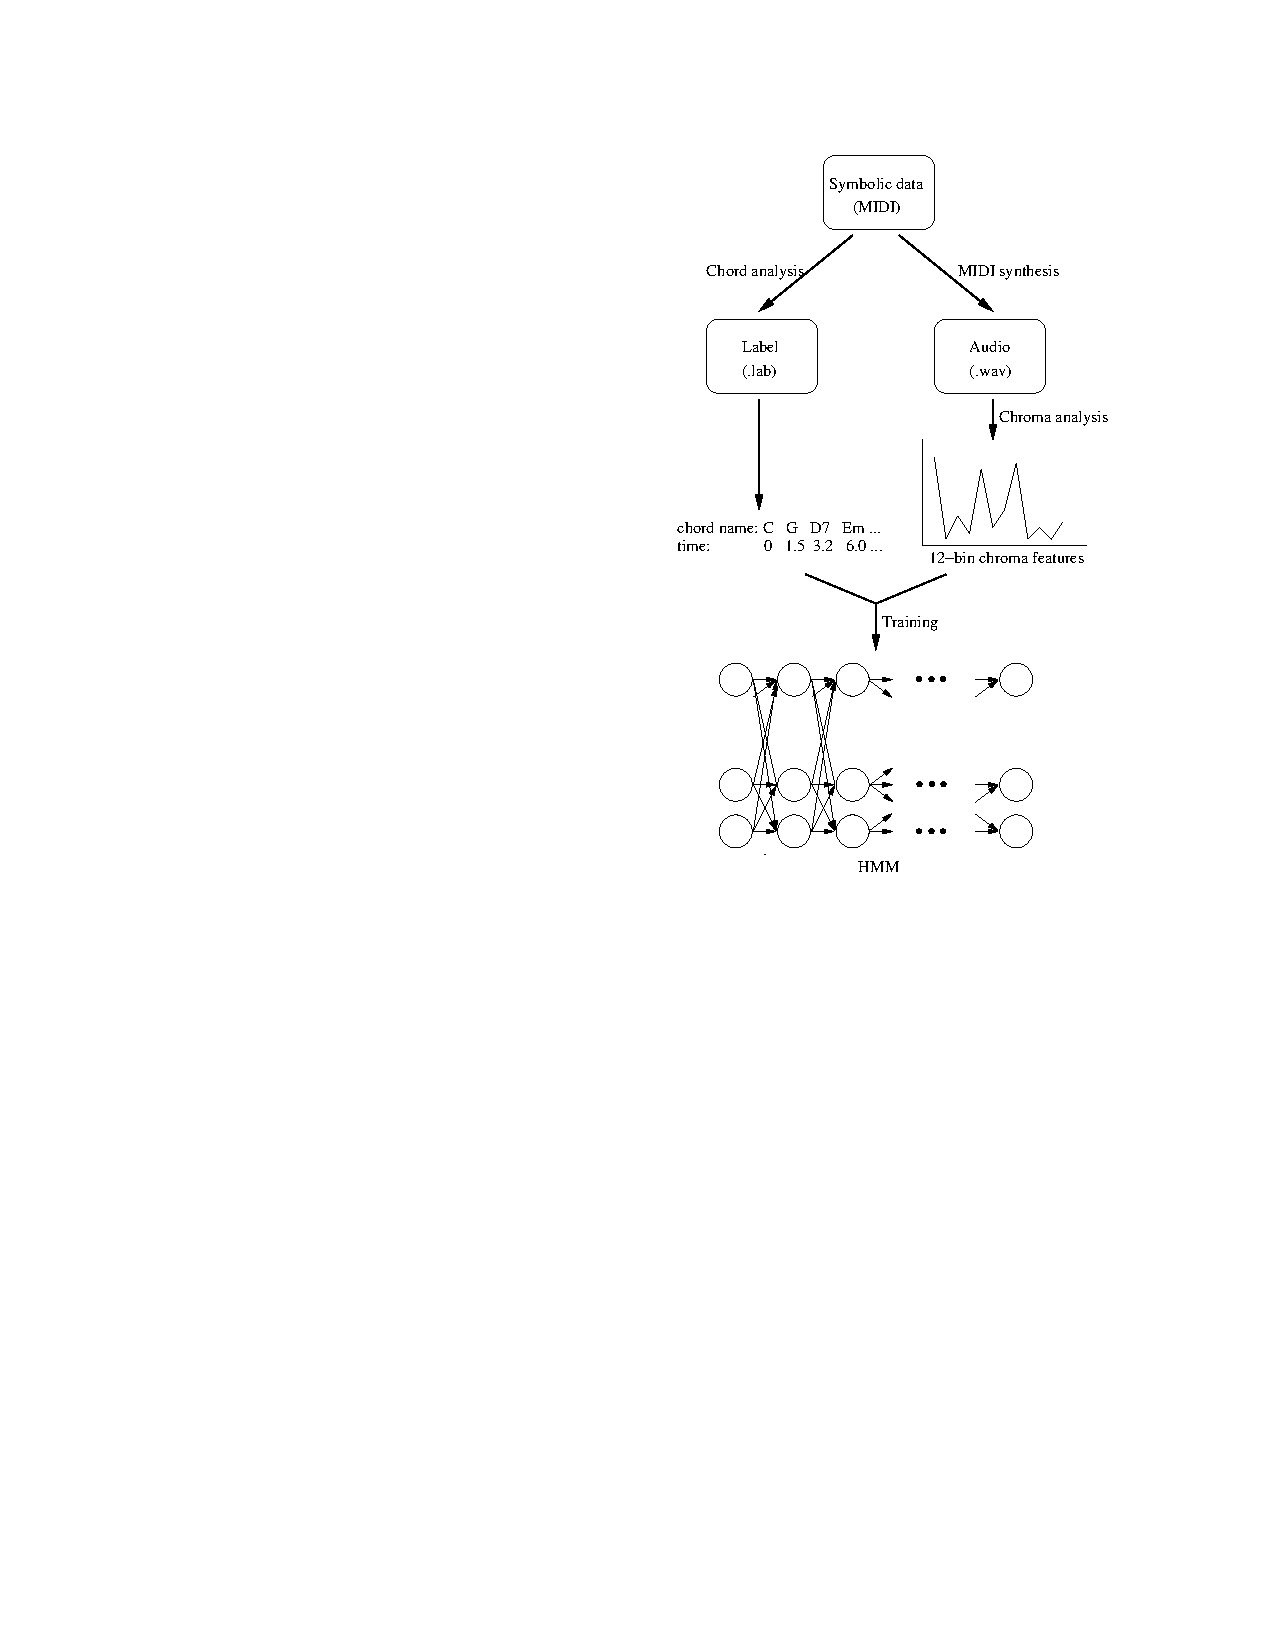
\includegraphics[height=.85\textheight]{fig1.pdf}
  	\end{column}
  	\end{columns}
\end{frame} 

\begin{frame}
	\frametitle{Datasets}
	\begin{itemize}
		\item Two training datasets: 81 solo piano pieces, 196 string quartets by J.S. Bach, Beethoven, Mozart, and Haydn.
		\item Two testing datasets: 5 solo piano pieces, 5 string quartets selected from the Kostka and Payne's book.
		\item All combinations of training and testing data were tried.
	\end{itemize}
	
\end{frame}  

\begin{frame}
	\frametitle{Results}
	
	\begin{table}\small
\centering
\begin{tabular}{|c|c|c|} \hline
\textbf{Training Data} & \textbf{Test Data} & \textbf{Recognition Rate} \\ \hline
Piano & Piano & 68.69 \\ \hline
String Quartet & Piano & 73.40 \\ \hline
Piano \& Strings & Piano & 74.41 \\ \hline
Piano & String Quartet & 79.35 \\ \hline
String Quartet & String Quartet & 79.76 \\ \hline
Piano \& Strings & String Quartet & \textbf{80.16} \\ \hline
\end{tabular}
\caption{Recognition results for all six possible training - test pairs in research case 2}
\label{tab:tab5}
\end{table}
\end{frame} 



\subsection[Case 3: Importance of Individual Components]{Case 3: Importance of Individual Components}

\begin{frame}
  \frametitle{Case 3: Importance of Individual Components}
    \begin{columns}
	\begin{column}{.6\textwidth}
	Four experiments:
	\begin{itemize}
		\item Using different combinations of preprocessing techniques during feature extraction.
		\item Pre-filtering using moving average filters, which look for noisy frames and smooth them across neighboring frames.
		\item Post-filtering using an HMM.
		\item Using both pre-filtering and post-filtering.
	\end{itemize}
	\end{column}
	\begin{column}{.4\textwidth}
  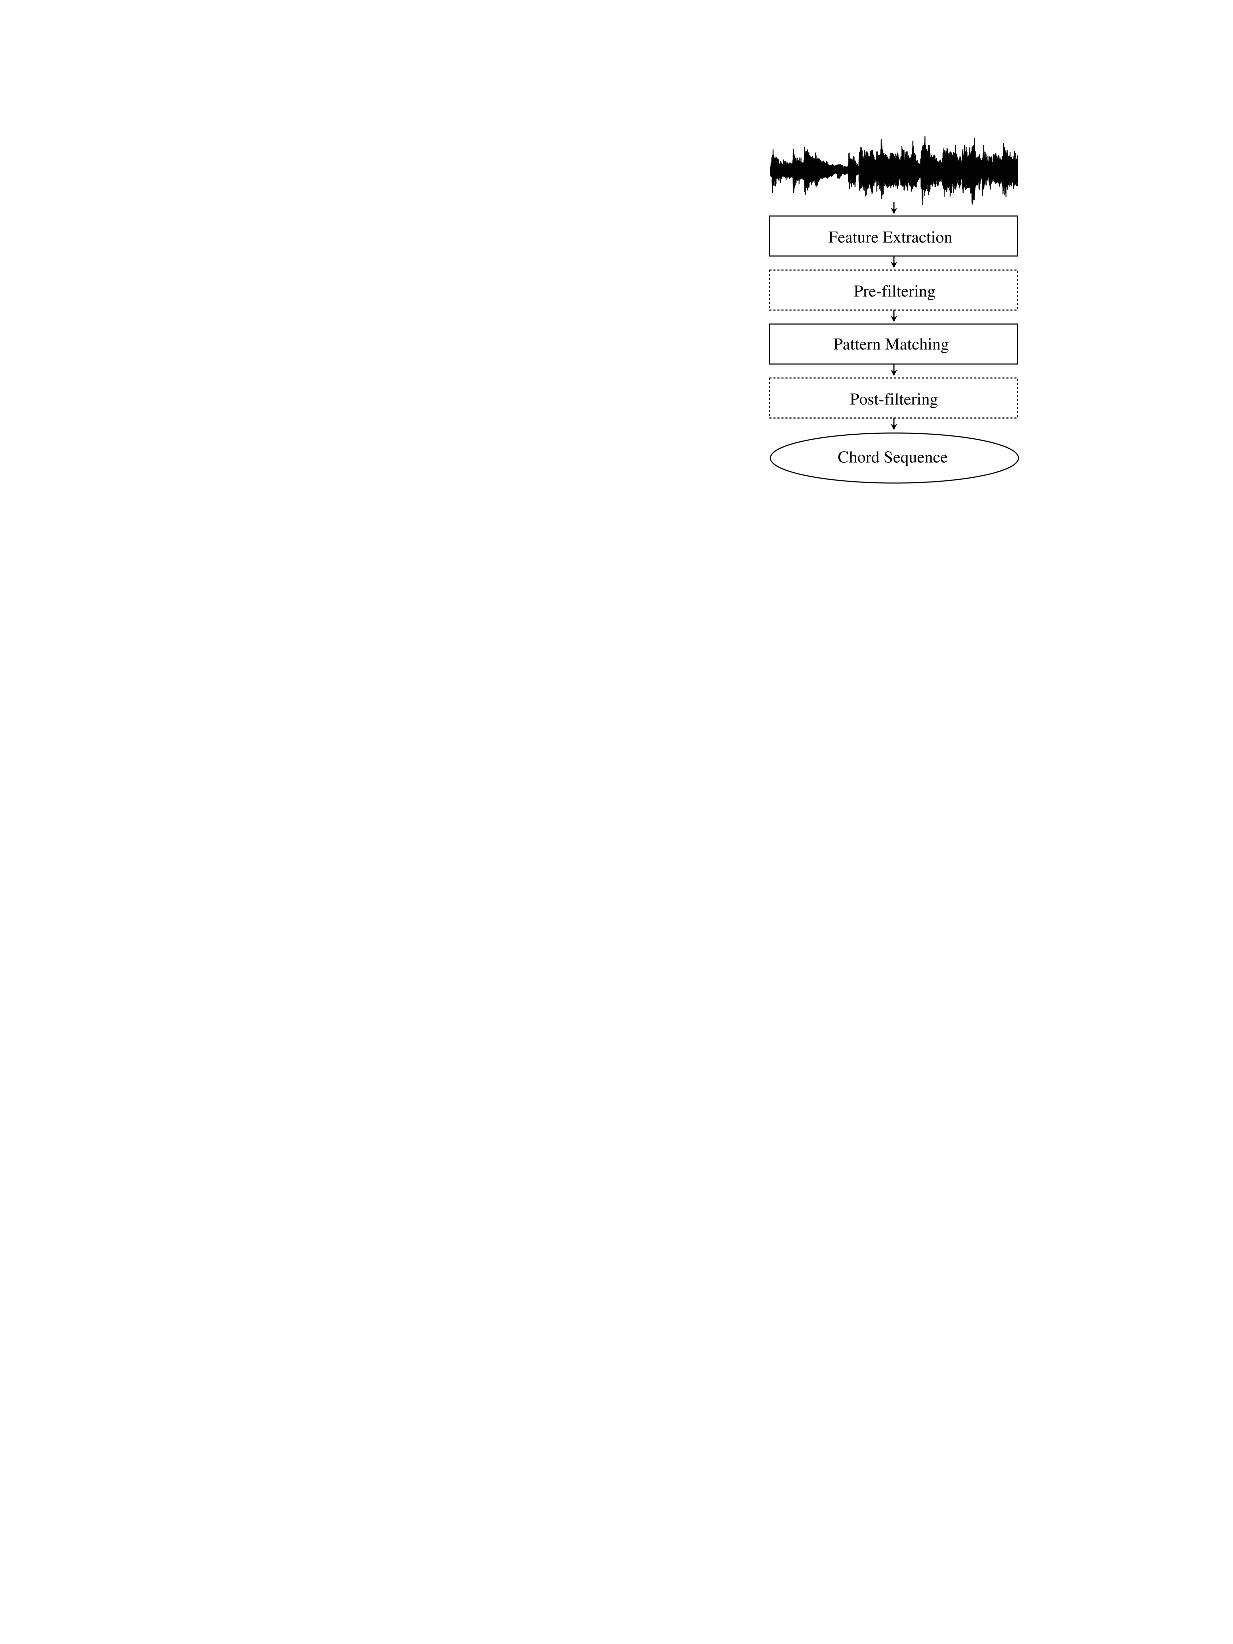
\includegraphics[width=.95\textwidth]{fig3.pdf}
  	\end{column}
  	\end{columns}
\end{frame}

\begin{frame}
	\frametitle{Datasets}
	\begin{itemize}
		\item Each experiment was performed on 495 chord labeled songs.
		\item 180 Beatles songs, 20 Queen songs, 100 songs from the Real World Computing (RWC) pop dataset, and 195 songs from the US-Pop dataset.
		\item 5 groups of 99 songs were selected randomly, with four used for training and one for testing.
	\end{itemize}
\end{frame}  

\begin{frame}
	\frametitle{Results}
	\begin{itemize}
	\item Each experiment was tried using 1, 5, 10, and 25 Gaussian components, with the best result shown.
	\item Increasing the number of components helped when using HMMs because they are dependent on transition probabilities.
	\item For preprocessing, high and low frequencies were de-emphasized and log compression was used, which limits dynamic range caused by different instruments and volumes.
\end{itemize}		
	
\begin{table}\tiny
\centering
\begin{tabular}{|c|c|c|c|c|} \hline
\textbf{Expt.} & \textbf{Highest Accuracy} & \textbf{Pre-filtering} & \textbf{Pattern Matching} & \textbf{Post-filtering} \\ \hline
1 & 58.30 & - & 1 Gaussian component & - \\ \hline
2 & 71.22 & Moving average filters & 1 Gaussian component & - \\ \hline
3 & \textbf{77.90} & - & 25 Gaussian components & HMM \\ \hline
4 & 77.58 & Moving average filters & 25 Gaussian components & HMM \\ \hline

\end{tabular}
\caption{Results from research case 3, showing the highest accuracy in each experiment, and the components used to achieve it}
\label{tab:tab9}
\end{table}

\end{frame}  


\section[Conclusions]{Conclusions}

\begin{frame}
	\frametitle{Conclusions}
	\begin{itemize}
		\item Isolated chords were more of a proof of concept.
		\item Highest accuracy is around 88\%, achieved using homomorphic liftering, HPS, chord segmentation, and SVMs for labeling.
		\item This system was dependent on the training data, and SVMs don't work as well for large datasets.
		\item Systems can be specifically tailored to type types of instruments and chords present in the dataset.
		\item Advances are being made in more general models that can provide chords for any given song.
	\end{itemize}
\end{frame}

\begin{frame}
	\frametitle{Thanks!}
	
	Thank you for your time and attention!
		
	\linespace
	\linespace
	
	Contact:  
	\begin{itemize}
		\item \texttt{emmon046@morris.umn.edu}
	\end{itemize}
	
	\linespace
	\linespace
	
	\begin{center}
	{\huge Questions?}
	\end{center}
\end{frame}

\section*{References}

\begin{frame}[allowframebreaks] 
	\frametitle{References} 
	
	\begin{thebibliography}{lskdjf}

\bibitem{Morman:2006}
Morman, Joshua and Rabiner, Lawrence.
\newblock A System for the Automatic Segmentation and Classification of Chord Sequences.
\newblock In Proceedings of the 1st ACM workshop on Audio and music computing multimedia (AMCMM '06). ACM, New York, NY, USA, 1-10. DOI=10.1145/1178723.1178725

\bibitem{Lee:2006}
Lee, Kyogu and Slaney, Malcolm
\newblock Automatic Chord Recognition from Audio Using a Supervised HMM Trained with Audio-from-symbolic Data.
\newblock In Proceedings of the 1st ACM workshop on Audio and music computing multimedia (AMCMM '06). ACM, New York, NY, USA, 11-20. DOI=10.1145/1178723.1178726 

\bibitem{TaeMin:2014}
TaeMin Cho and Bello, J.P.
\newblock On the Relative Importance of Individual Components of Chord Recognition Systems.
\newblock IEEE/ACM Trans. Audio, Speech and Lang. Proc. 22, 2 (February 2014), 477-492. DOI=10.1109/TASLP.2013.2295926 

\bibitem{McVicar:2014}
McVicar, M. and Santos-Rodriguez, R. and Yizhao Ni and Tijl De Bie
\newblock Automatic Chord Estimation from Audio: A Review of the State of the Art
\newblock IEEE/ACM Trans. Audio, Speech and Lang. Proc. 22, 2 (February 2014), 556-575. DOI=10.1109/TASLP.2013.2294580 
  
  	\end{thebibliography}

\end{frame} 

\end{document}


